%%
%% ****** ljmsamp.tex 13.06.2018 ******
%%
\documentclass[
11pt,%
tightenlines,%
twoside,%
onecolumn,%
nofloats,%
nobibnotes,%
nofootinbib,%
superscriptaddress,%
noshowpacs,%
centertags]%
{revtex4}
\usepackage{ljm}
\usepackage{listings}
\usepackage{amsmath,amsthm,amscd,amsfonts,amssymb}
\usepackage{textcomp}
\usepackage{graphicx}
\usepackage{esvect}
\usepackage{physics}

\lstset{
language=C++,
basewidth=0.5em,
xleftmargin=45pt,
xrightmargin=45pt,
basicstyle=\small\ttfamily,
keywordstyle=\bfseries\underbar,
numbers=left,
numberstyle=\tiny,
stepnumber=1,
numbersep=10pt,
showspaces=false,
showstringspaces=false,
showtabs=false,
frame=trBL,
tabsize=2,
captionpos=t,
breaklines=true,
breakatwhitespace=false,
escapeinside={\%*}{*)}
}

\begin{document}

\titlerunning{TODO : RUNNING TITLE} % for running heads
\authorrunning{A.~A.~Rybakov and S.~S.~Shumilin} % for running heads
%\authorrunning{First-Author, Second-Author} % for running heads

\title{TODO : FULL TITLE}
% Splitting into lines is performed by the command \\
% The title is written in accordance with the rules of capitalization.

\author{\firstname{A.~A.}~\surname{Rybakov}}
\email[E-mail: ]{rybakov.aax@gmail.com} \affiliation{Joint
Supercomputer Center of the Russian Academy of Sciences (JSCC RAS)
-- Branch of Scientific Research Institute of System Analysis of the
Russian Academy of Sciences, Leninsky prospect 32a, Moscow, 119334,
Russia}

\author{\firstname{S.~S.}~\surname{Shumilin}}
\email[E-mail: ]{shumilin@jscc.ru} \affiliation{Joint Supercomputer
Center of the Russian Academy of Sciences (JSCC RAS) -- Branch of
Scientific Research Institute of System Analysis of the Russian
Academy of Sciences, Leninsky prospect 32a, Moscow, 119334, Russia}
%\noaffiliation % If the author does not specify a place of work.

\firstcollaboration{(Submitted by TODO : SUBMITTER)} % Add if you know submitter.
%\lastcollaboration{ }

\received{TODO : DATE} % The date of receipt to the editor, i.e. December 06, 2017

\begin{abstract}
TODO : ABSTRACT
\end{abstract}

\subclass{TODO : CODE} % Enter 2010 Mathematics Subject Classification.

\keywords{TODO : KEYWORDS} % Include keywords separeted by comma.

\maketitle

% Text of article starts here.

\section{Introduction}

TODO : INTRODUCTION

\section{Решение задачи о перестроении двумерной поверхности}

Рассмотрим геометрическую задачу о перестроении двумерной поверхности в общем виде.
Пусть даны $n$ ячеек двумерной поверхностной сетки, каждая из которых представлена отрезком длины $l_i$ (то есть общее количество узлов равно $n + 1$).
Известно направление изменения поверхности каждой ячейки (направление нормали к отрезку), а также направление движения каждого узла (совпадает с направлением суммы единичных нормалей, проведенных к инцидентным ячейкам) (Fig.~\ref{fig:grid_normals}).

\begin{figure}[h]
\setcaptionmargin{5mm}
\onelinecaptionstrue
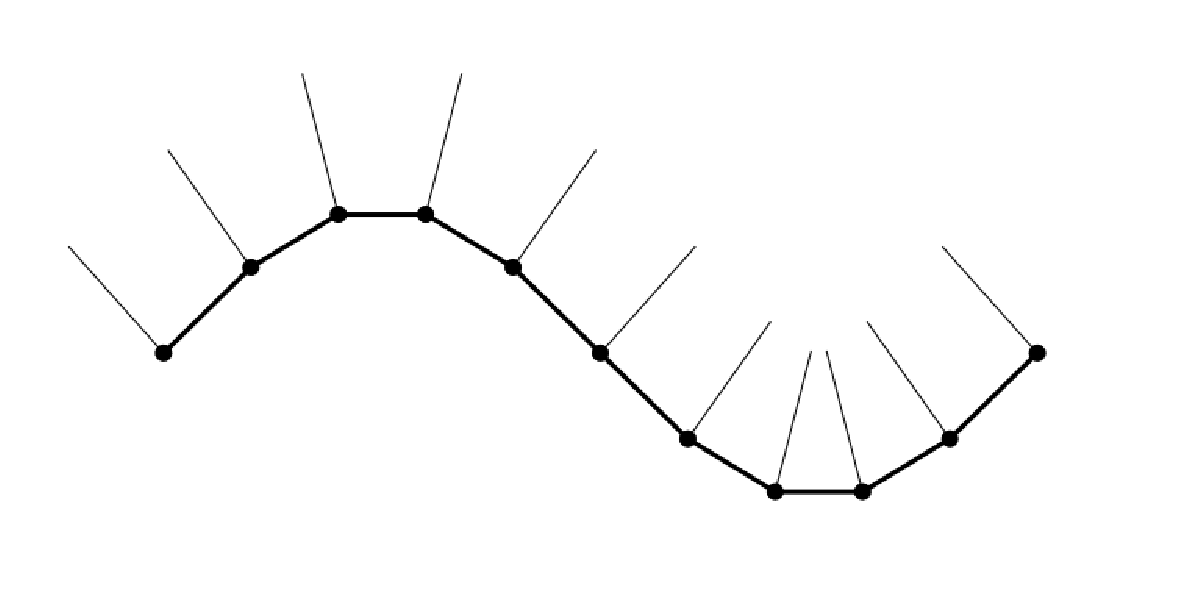
\includegraphics[width=0.8\textwidth]{pics/grid_normals.pdf}
\captionstyle{normal}\caption{Двумерная поверхностная сетка с обозначенными направлениями движения узлов.}
\label{fig:grid_normals}
\end{figure}

Также известны локальные сдвиги поверхности для каждой ячейки (они задаются значениями $H_i$).
Требуется найти такие значения локальных сдвигов узлов сетки $h_i$, чтобы охватывающая площадь между старой поверхностью и новой поверхностью для каждой ячейки сетки ($S_i$) как можно меньше отличалась от требуемого значения $T_i = l_iH_i$.

Для решения данной задачи сначала требуется вычислить охватывающую площадь для каждой отдельной ячейки.

\subsection{Задача о вычислении охватывающей площади при движении узлов отдельной ячейки}

Рассматривается ячейка, представленная на плоскости отрезком $AB$ длины $l$.
При перемещении точек $A$ и $B$ в новые точки $A_1$ и $B_1$ соответственно образуется четырехугольник $AA_1B_1B$.
Требуется найти его площадь, выраженную явно через параметры $a = \overline{AA_1}$ и $b = \overline{BB_1}$ (Fig.~\ref{fig:local}).

\begin{figure}[h]
\setcaptionmargin{5mm}
\onelinecaptionstrue
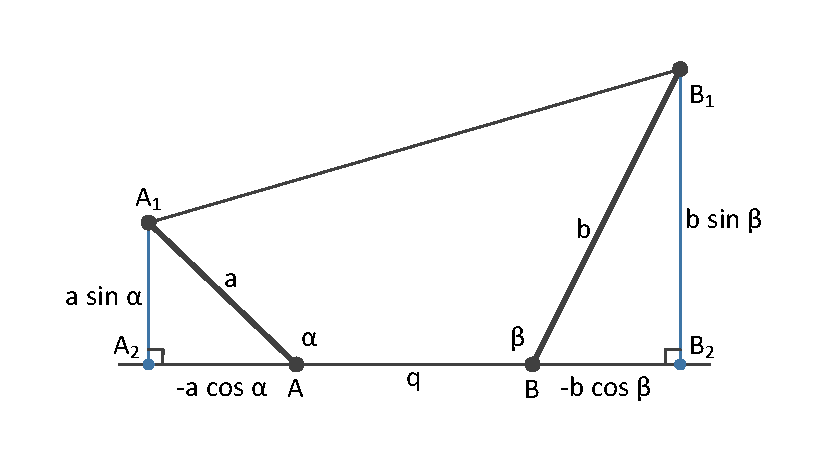
\includegraphics[width=0.8\textwidth]{pics/local.pdf}
\captionstyle{normal}\caption{Вычисление охватывающей площади при передвижении узлов ячейки.}
\label{fig:local}
\end{figure}

Для решения задачи опустим перпендикуляры из точек $A_1$ и $B_1$ на прямую $AB$.
Их основаниями будут точки $A_2$ и $B_2$ соответственно.
Искомая площадь может быть представлена в следующем виде:

\begin{equation}
S_{AA_1B_1B} = S_{A_2A_1B_1B_2} - S_{AA_1A_2} - S_{BB_1B_2}
\end{equation}

Обозначим угол между векторами $\overline{AA_1}$ и $\overline{AB}$ через $\alpha$, а угол между векторами $\overline{BB_1}$ и $\overline{BA}$ через $\beta$.
Тогда искомая площадь вычисляется явно в следующем виде:

\begin{equation}
S_{AA_1B_1B} = \frac{1}{2}(l - a \cos \alpha - b \cos \beta)(a \sin \alpha + b \sin \beta) + \frac{1}{2}a^2 \sin \alpha \cos \alpha + \frac{1}{2}b^2 \sin \beta \cos \beta
\end{equation}

\begin{equation}
S_{AA_1B_1B} = \frac{1}{2}\big(l(a \sin \alpha + b \sin \beta) - ab \sin(\alpha + \beta)\big)
\end{equation}

\subsection{Решение методом градиентного спуска}

Метод градиентного спуска является наиболее простым методом оптимизации.
При условии, что в любой точки функции можно вычислить ее градиент, то начиная с некоторого начального приближения $x_0$ строится итерационная последовательность~\cite{Polyak}:

\begin{equation}
x^{k+1} = x^k - \gamma _k \nabla f(x_k)
\end{equation}

где $\gamma _k \geq 0$ задает длину шага и, соответственно, скорость градиентного спуска.
Градиентный метод находит свое основное применение в задаче поиска минимума или максимума функции.
Направление антиградиента является направлением наискорейшего убывания функции.
В процессе выполнения операций критериями останова являются сходимость по аргументу, по значению функции или по норме вектора градиента.

\begin{equation}
|x^{k+1} - x^k| \leq \varepsilon,
\end{equation}

\begin{equation}
|f(x^{k+1})- f(x^k)| \leq \varepsilon,
\end{equation}

\begin{equation}
||\nabla f(x^{k+1})|| \leq \varepsilon
\end{equation}


Рассмотрим решение поставленной задачи методом градиентного спуска.
Неизвестными параметрами являются величины сдвигов узлов сетки $h_i$.
Опираясь на решение локальной задачи об определении охватывающей площади можно записать охватывающую площадь при движении отдельной ячейки:

\begin{equation}
S_i = \frac{1}{2}\big(l_i(h_i \sin \alpha_i + h_{i + 1} \sin \beta_i) - h_ih_{i + 1} \sin(\alpha_i + \beta_i)\big) 
\end{equation}

Тогда ошибку определения охватывающей площади в ячейке будем определять как $\delta_i = (S_i - T_i)^2$.
Общая ошибка при перестроении поверхности задается как среднее значение ошибок для всех ячеек:

\begin{equation}
\epsilon = \frac{1}{n}\sum_{i = 0}^{n - 1}{\delta_i}
\end{equation}

\begin{equation}
\frac{\partial \epsilon}{\partial h_i} = \frac{1}{n}\big(\frac{\partial \delta_{i - 1}}{\partial h_i} + \frac{\partial \delta_i}{\partial h_i}\big)
\end{equation}

где

\begin{equation}
\begin{cases}
\frac{\partial \delta_{i - 1}}{\partial h_i} = (S_{i - 1} - T_{i - 1})(l_{i - 1} \sin \beta_{i - 1} - h_{i - 1} \sin(\alpha_{i - 1} + \beta_{i - 1})) \\
\frac{\partial \delta_i}{\partial h_i} = (S_i - T_i)(l_i \sin \alpha_i - h_{i + 1} \sin(\alpha_i + \beta_i))
\end{cases}
\end{equation}

\section{Схемы приближенного решения}

TODO : SECTION 3

\subsection{Решение методом прямоугольников}

\begin{figure}[h]
\setcaptionmargin{5mm}
\onelinecaptionstrue
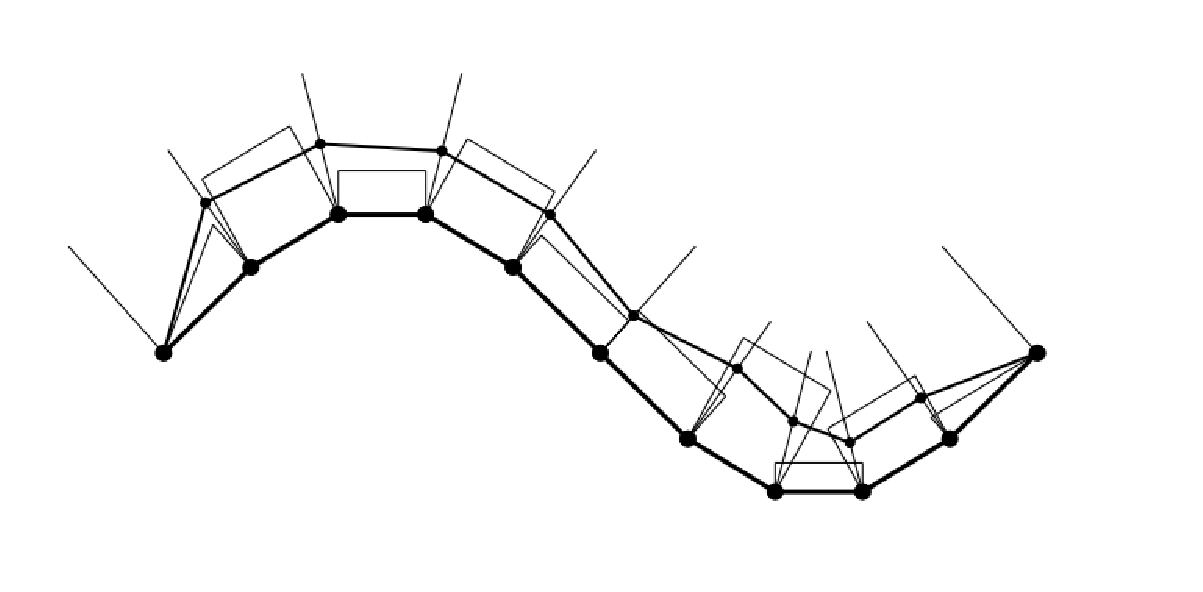
\includegraphics[width=0.8\textwidth]{pics/grid_rectangles.pdf}
\captionstyle{normal}\caption{Перестроение поверхности методом прямоугольников.}
\label{fig:grid_rectangles}
\end{figure}

\subsection{Решение методом трапеций}

\begin{figure}[h]
\setcaptionmargin{5mm}
\onelinecaptionstrue
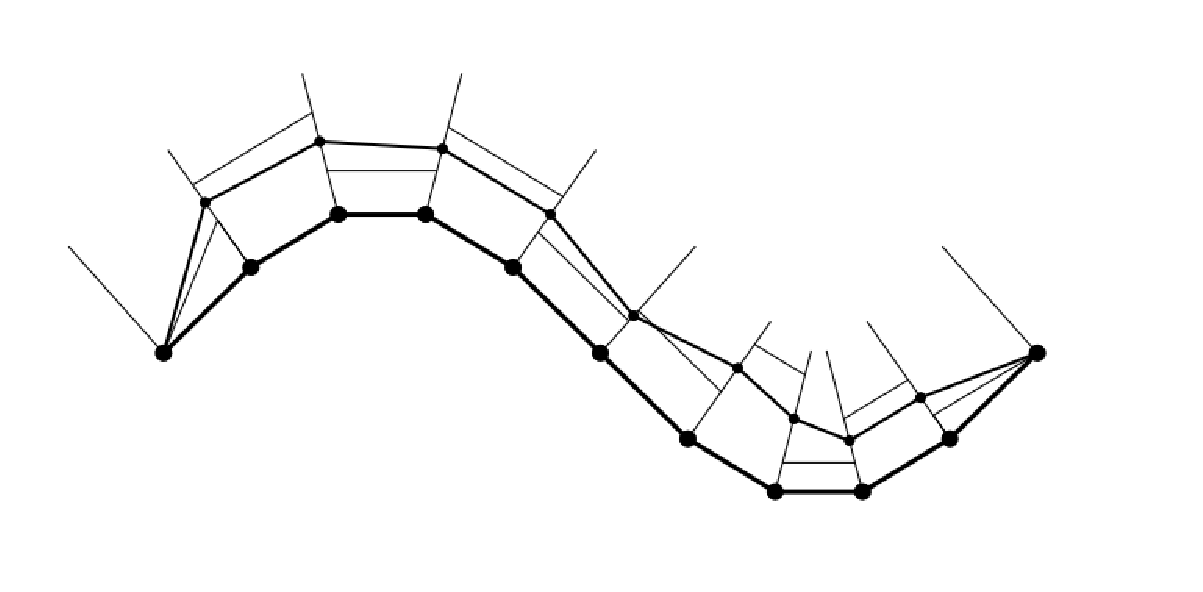
\includegraphics[width=0.8\textwidth]{pics/grid_trapeziums.pdf}
\captionstyle{normal}\caption{Перестроение поверхности методом трапеций.}
\label{fig:grid_trapeziums}
\end{figure}

\section{Conclusion}

TODO : CONCLUSION

\begin{acknowledgments}
The work has been done at the JSCC RAS as part of the state assignment for the topic 0065-2019-0016 (reg. no. AAAA-A19-119011590098-8). The supercomputer MVS-10P, located at the JSCC RAS, was used for calculations during the research.
\end{acknowledgments}

\begin{thebibliography}{99}

% References for INTRODUCTION section.

\bibitem{Rettinger}
\refitem{article}
C. Rettinger, C. Godenschwager, S. Eibl, et al., {\it ``Fully Resolved Simulations of Dune Formation in Riverbeds"}, ISC High Performance , LNCS~{\bf 10266}, 3--21 (2017).
\bibitem{Polyak}
\refitem{book}
Polyak B.T. Vvedenie v optimizaciyu. Moscow, Nauka, 1983, 384 p.

\end{thebibliography}

\end{document}
